\documentclass{article}
\usepackage{graphicx}

\begin{document}

\title{
	\huge{ET2440}
	\linebreak
	\linebreak
	BUTP protocol design and implementation
}
\date{\today}

\author{Alexander Rajula}

\maketitle

\newpage
\section{Protocol description}
The BUTP protocol is a transport-layer protocol designed to enable reliable transmission of data over unreliable physical media. It sits on top of UDP in the TCP/IP protocol suite, but can with a few modifications be made to sit on top of IP itself (raw sockets). The protocol implements two techniques for managing transmission window size and packet timeout and retransmission control. BUTP is elementary in its design, and does not implement, for instance maximum path MTU discovery, as specified in RFC 1191 for IPv4 and RFC 1981 for IPv6.

\subsection{The BUTP protocol header}
The BUTP protocol header consists of a fixed and a variable part. The fixed part must always be present. The header is shown in Fig. 1 below.

\begin{center}
        \begin{figure}[h!]
        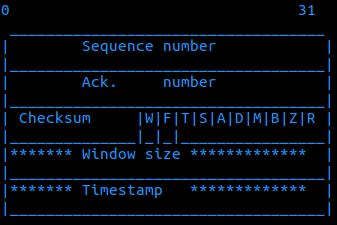
\includegraphics[width=125mm]{butp_header.png}
        \caption{BUTP protocol header}
        \end{figure}
\end{center}

\subsubsection{Sequence numbers}
In BUTP, each outgoing packet is tagged with a unique (modulo $2^{32}$) sequence number. The sequence number grows with the number of data bytes sent in each packet, so that the sequence number is always increasing (until wraparound). If data is sent, the DATA flag is set.

\subsubsection{Acknowledgement numbers}
In BUTP, in contrast to TCP, a recipient acknowledges packages by setting the ACK flag in a packet and inserting the sequence number of the incoming packet into the outgoing packet.

\subsubsection{Checksum}
To facilitate corruption-free data delivery, a 16-bit checksum is calculated as specified in RFC 793.

\subsubsection{Options}
BUTP uses many flags to simplify the protocol and implementation. We list them here, in order:
\begin{itemize}
  \item W - Window flag, sender of this packet pushes window information
  \item F - Finished flag, sender has sent all of its data, and received ACKs for all its data
  \item T - Timestamp flag, packet contains a timestamp
  \item S - Synchronization flag, packet indicates that the connection should be reset (or initiated)
  \item A - Acknowledgement flag, packet contains an acknowledgement for a packet previously sent
  \item D - Data flag, packet contains application-layer data
  \item M - My timestamp flag, if set this means that the timestamp was set by the sender of this packet, and should be echoed in a response packet
  \item B - Abort flag, connection should be aborted and any undelivered data should be cleared from buffers
  \item Z - Finished and acknowledged flag, this flag is set in response to a finished flag.
\end{itemize}

\subsubsection{Window}
If the window flag is set, this field contains window information from the sender which MUST be obeyed.

\subsubsection{Timestamp}
If the timestamp flag is set, this field contains a timestamp set by either sender or receiver, depending on whether the M flag is set. It is used to calculate round-trip-time, which in turn is used to set an upper bound for how long the protocol should wait before re-transmitting a previously transmitted packet.

\subsection{Connection establishment}
To establish a connection between two hosts, BUTP uses a three-way handshake, in the same manner as TCP.

\subsection{Calculation of round-trip-time}
The protocol uses the timestamp field to calculate the path round-trip time. This value is used to set an upper bound for how long a packet can be in transit without being acknowledged. There is no fixed time interval between timestamp measurements, it is up to the implementation.

\subsection{Growing and shrinking window}
In the three-way handshake, both hosts communicate initial window sizes. This window size is then changed by the protocol in response to acknowledgements and timeouts. If an ack is received, the window grows. If a packet's timeout expires and has to be re-transmitted, the window shrinks. The purpose of this system is to control the number of packets (and thus bytes) in transit at once in the network between sender and receiver. If the number of bytes in transit equals the window size, the protocol has to wait until packets are acknowledged before it can continue sending data (re-transmissions do not respect this since the ACK timer expires, the packets in transit for which it expired are considered lost).

\section{Notes on the implementation}
The implementation of the BUTP protocol described herein is written in the C programming language using UNIX sockets for network communications, and also uses Linux system libraries. It is thus confined to the Linux operating system. Two test programs are included, \texttt{server.c} and \texttt{client.c}, and they can be built by executing the \texttt{build.sh} script. The server has to be started before the client for the three-way handshake to work.  The test programs each transmit an image to the other part, simultaneously. The packet loss ratio is set by the user at client/server startup, to simulate a lossy transmission line.
\subsection{The server program}
When run, the server asks for a port number to which it will bind an unconnected datagram socket, and the packet loss ratio (for simulation purposes). One then has the option to choose if one wants to listen on IPv4 or IPv6 (this has implications for communication with the other host, both hosts must use the same network-layer protocol).

\subsection{The client program}
The server ip address and port number, as well as the packet loss ratio, is specified as arguments to the client program at startup as follows:\newline
\texttt{./client rajula.org 11337 25}

\subsection{Simulating packet loss}
As described above, packet loss simulation is controlled by specifying the packet loss ratio for the client and server at program startup.

\subsection{Shrinking and growing window}
The protocol implementation is as simple as can be with regards to shrinking and growing the window for the amount of bytes which can be in transit at once. The protocol simply increases the window by a fixed amount if an ACK for a previously sent packet is received, and decreases the window by a fixed amount if a packet has to be re-transmitted.

\subsection{Calculation of ACK timeout}
The implementation is quite flexible with regards to packet timeout adjustment. In its current state, the implementation sets the timeout value to four times that of the calculated round-trip time. In this way, the ack timeout is continuously changed in response to updated round-trip time measurements.

\subsection{Measurement of round-trip time}
The round-trip time measurement is quite simple. The decision on whether to include a timestamp in a packet is random. A timestamp is calculated based on the computer clock, and when the timestamp bounces back, that same timestamp is used to calculate the time difference between current time and the timestamp.

\subsection{Data transmission between client and server test programs}
The client and server test applications each have two \texttt{JPEG} images, \texttt{servercat.jpg} and \texttt{clientdog.jpg}, respectively. The test programs load the images into memory and push the data onto the transport layer (BUTP). BUTP takes care of the data transmission and also writes the received data to a file called \texttt{received.jpg}.

\subsection{Future implementation improvements}
The protocol ought to run in its separate thread in kernel space - this is not implemented, it runs in the server and client application threads as a set of functions.\newline
To have a useable interface, one should be able to push and pull data to the transport layer seamlessly (this is almost implemented at this time, minor adjustments are needed).

\subsection{Application-layer programming interface}
There are currently a few number of functions calls to the transport layer protocol:
\begin{itemize}
  \item \texttt{int set\_parameters(struct addrinfo* dest, uint8\_t packet\_loss\_ratio)} - Initializes variables and sets destination address
  \item \texttt{int yell()} - Call from client to server to initiate three-way handshake
  \item \texttt{int yawn()} - Tell transport layer to begin listening for incoming three-way handshake
  \item \texttt{int push(const char* buf, const int buflen)} - Push application-layer data to transport layer
  \item \texttt{int pull(char* buf, uint32\_t buflen)} - Pull transport layer data up to applicaiton layer (if any)
  \item \texttt{void loop()} - Initializes transport protocol (never exits in current application - program has to be terminated with \texttt{CTRL-C}
\end{itemize}

\subsection{Tuning BUTP}
There is great flexibility in tuning the operation of BUTP for optimal data transmission. The algorithm for transmission window size (in the implementation stored in the \texttt{your\_win} variable) needs adjustment, since it is currently the simplest possible algorithm imaginable. Also, the calculation for RTT might be optimized, for instance by using some kind of smoothing operation, like calculating the running average over a long period to smooth out peaks and troughs in transmission delay.
\newline
\indent Compared to TCP, BUTP has no sophisticated slow-start algorithms or fast recovery procedures, although it could be implemented, and the amount of effort required lies mostly in figuring out the optimal algorithm.

\end{document}
